\documentclass{beamer}
\usetheme{Boadilla}
\usepackage{havannah}

\title[Learning MCTS]{Evolutionary Learning of Policies for MCTS Simulations}
\author[Pettit, Helmbold]{James Pettit, David Helmbold}
\institute[UCSC]{
  University of California, Santa Cruz\\
  \texttt{jpettit@soe.ucsc.edu}
}
\date[July 2012]{July 2012}

\begin{document}

\begin{frame}[plain]
  \titlepage
\end{frame}

\begin{frame}{Overview}
\begin{enumerate}
	\item The Game of Hex
	\item Monte-Carlo Tree Search (MCTS)
	\item Apply Evolutionary Learningto MCTS+Hex
	\item Results and Future Work
\end{enumerate}
\end{frame}

\begin{frame}{The Game of Hex}
\begin{itemize}
	\item 2 player, perfect information
	\item 6-sided hexagons on a parallelogram board
	\item Common sizes: 11, 13
\end{itemize}
\end{frame}

\begin{frame}{The Game of Hex - Example Board}
% example board, play a few moves, show final position
	\begin{figure}[tb]
	\resizebox{3.3in}{!}{ \begin{HexBoard}[board size=7]
		  \HGame{d4,d3,e3,f1,c2,d6,b5,e2,c4,c3,a4,b6,c6,c5,d5,b7,c7,b4,a5,b3,a3,b1,b2,c1,d1}
		\end{HexBoard}
		}
	\end{figure}
\end{frame}

\begin{frame}{The Game of Hex - Good for AI}
\begin{itemize}
	\item Easy to program
	\item Clear-cut winning condition
	\item Large problem space
	\item Solved for boards up to 7x7
\end{itemize}
\end{frame}

\begin{frame}{Tree Search}
\begin{itemize}
	\item Game tree grows exponentially
	\item Symmetry can halve space
	\item Limited opportunities for provable pruning
	\item No good position ranking heuristic
\end{itemize}
\end{frame}

\begin{frame}{Monte Carlo Tree Search}
\begin{itemize}
	\item Use random playouts to estimate minimax value
	\item Large enough playouts will converge to true minimax value
	\item Seems dumb, actually works
	\item Computationally very expensive
\end{itemize}
\end{frame}

\begin{frame}{Monte Carlo Tree Search - Playout Policy}
\begin{itemize}
	\item Naively ``improving'' the strength of the playout policy can hurt overall performance
	\item Requires careful and expensive testing to verify improvement
\end{itemize}
\end{frame}

\begin{frame}{Evolutionary Learning (Hivemind)}
\begin{itemize}
	\item Idea: Evolve playout policy
	\item Individual policies compete in a tournament to reproduce
	\item Self-play yields a self-bootstrapping system
\end{itemize}
\end{frame}

\begin{frame}{Evolution}
\begin{enumerate}
	\item Generate $n$ individuals (population)
	\item Evaluate fitness\label{eval}
	\item Rank by fitness
	\item Select top $c$ children, $c < n$
	\item Recombine children into $n$ new individuals (next generation)
	\item Mutate population
	\item Repeat from \ref{eval}
\end{enumerate}
\end{frame}

\begin{frame}{Encoding}
\begin{itemize}
	\item Individual policy is a collection of evolvable weights
	\item One weight, many interpretations
	\item Explicitly requires domain knowledge
	\item Implicitly limits the system
\end{itemize}
\end{frame}

\begin{frame}{Encoding - Example}
\begin{figure}
  \begin{center}
  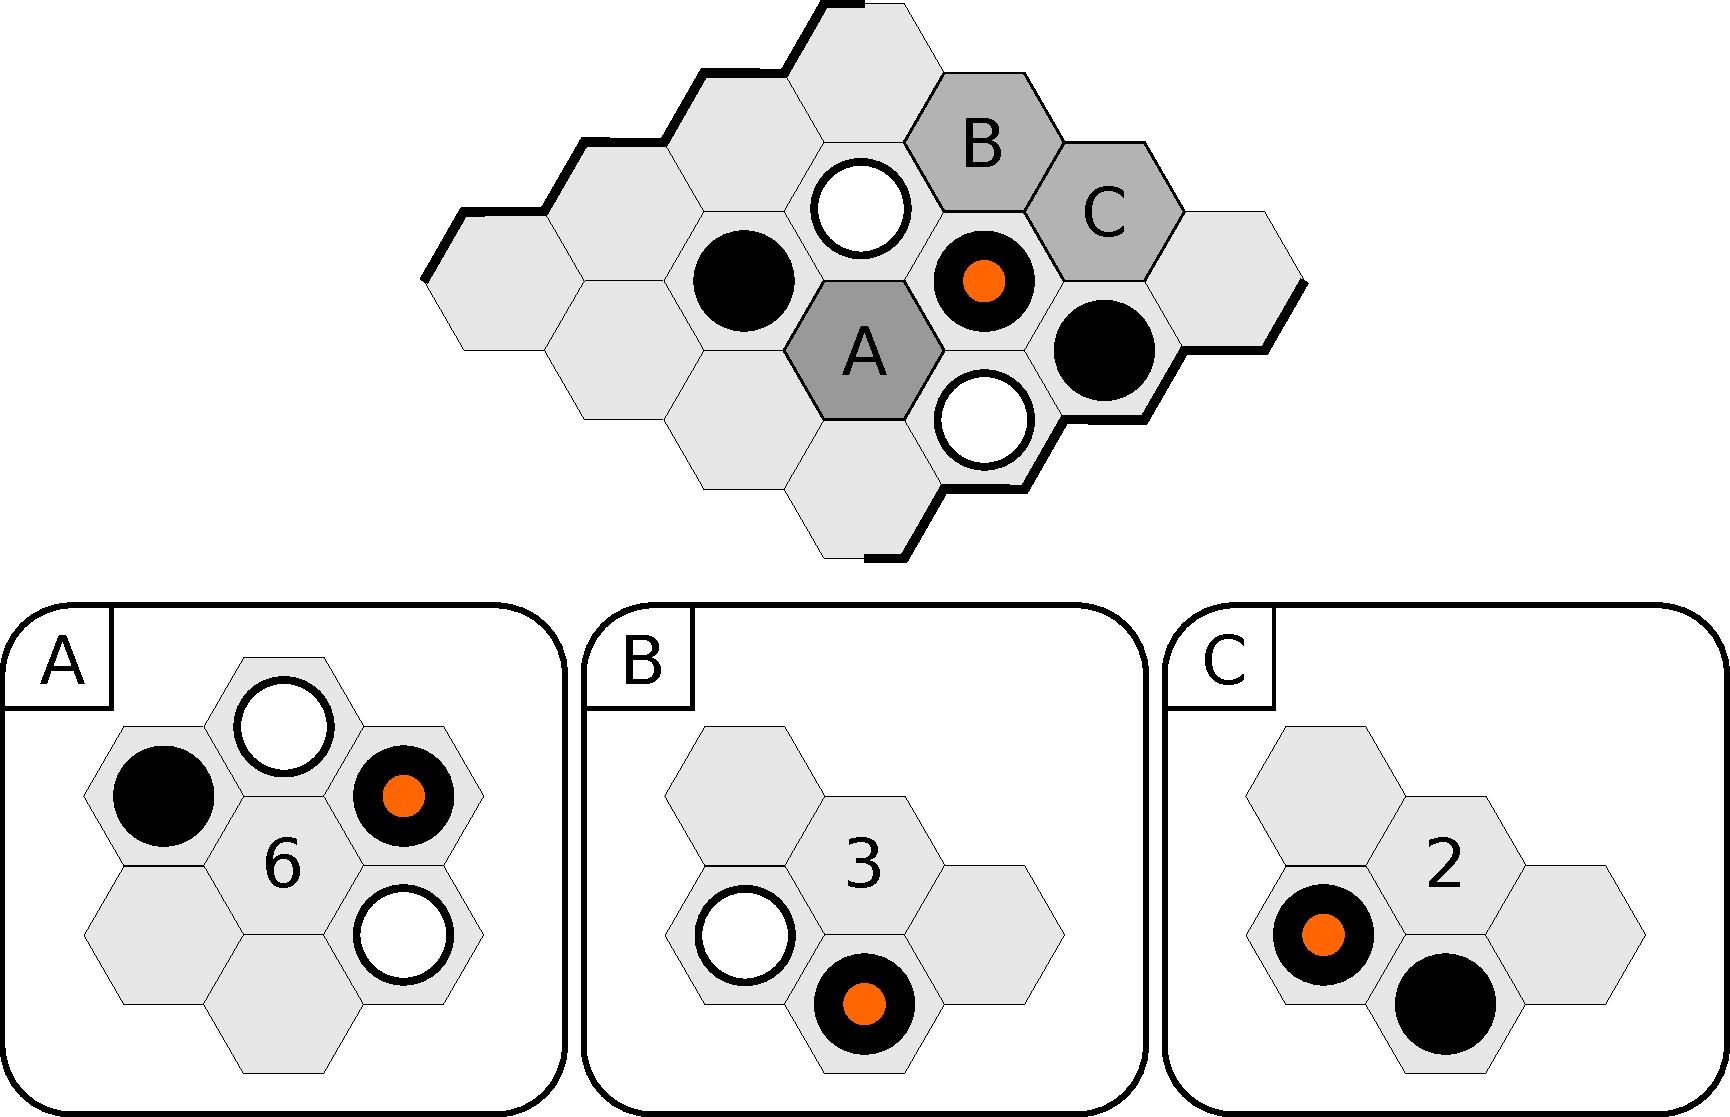
\includegraphics[width=3.25in]{graphics/local-pattern.pdf}
  \label{fig:encoding}
  \end{center}
\end{figure}
\begin{itemize}
	\item Weight moves local to last-played move
	\item If local area is filled, use default policy
\end{itemize}
\end{frame}

\begin{frame}{Encoding - Example}
\begin{figure}
  \begin{center}
  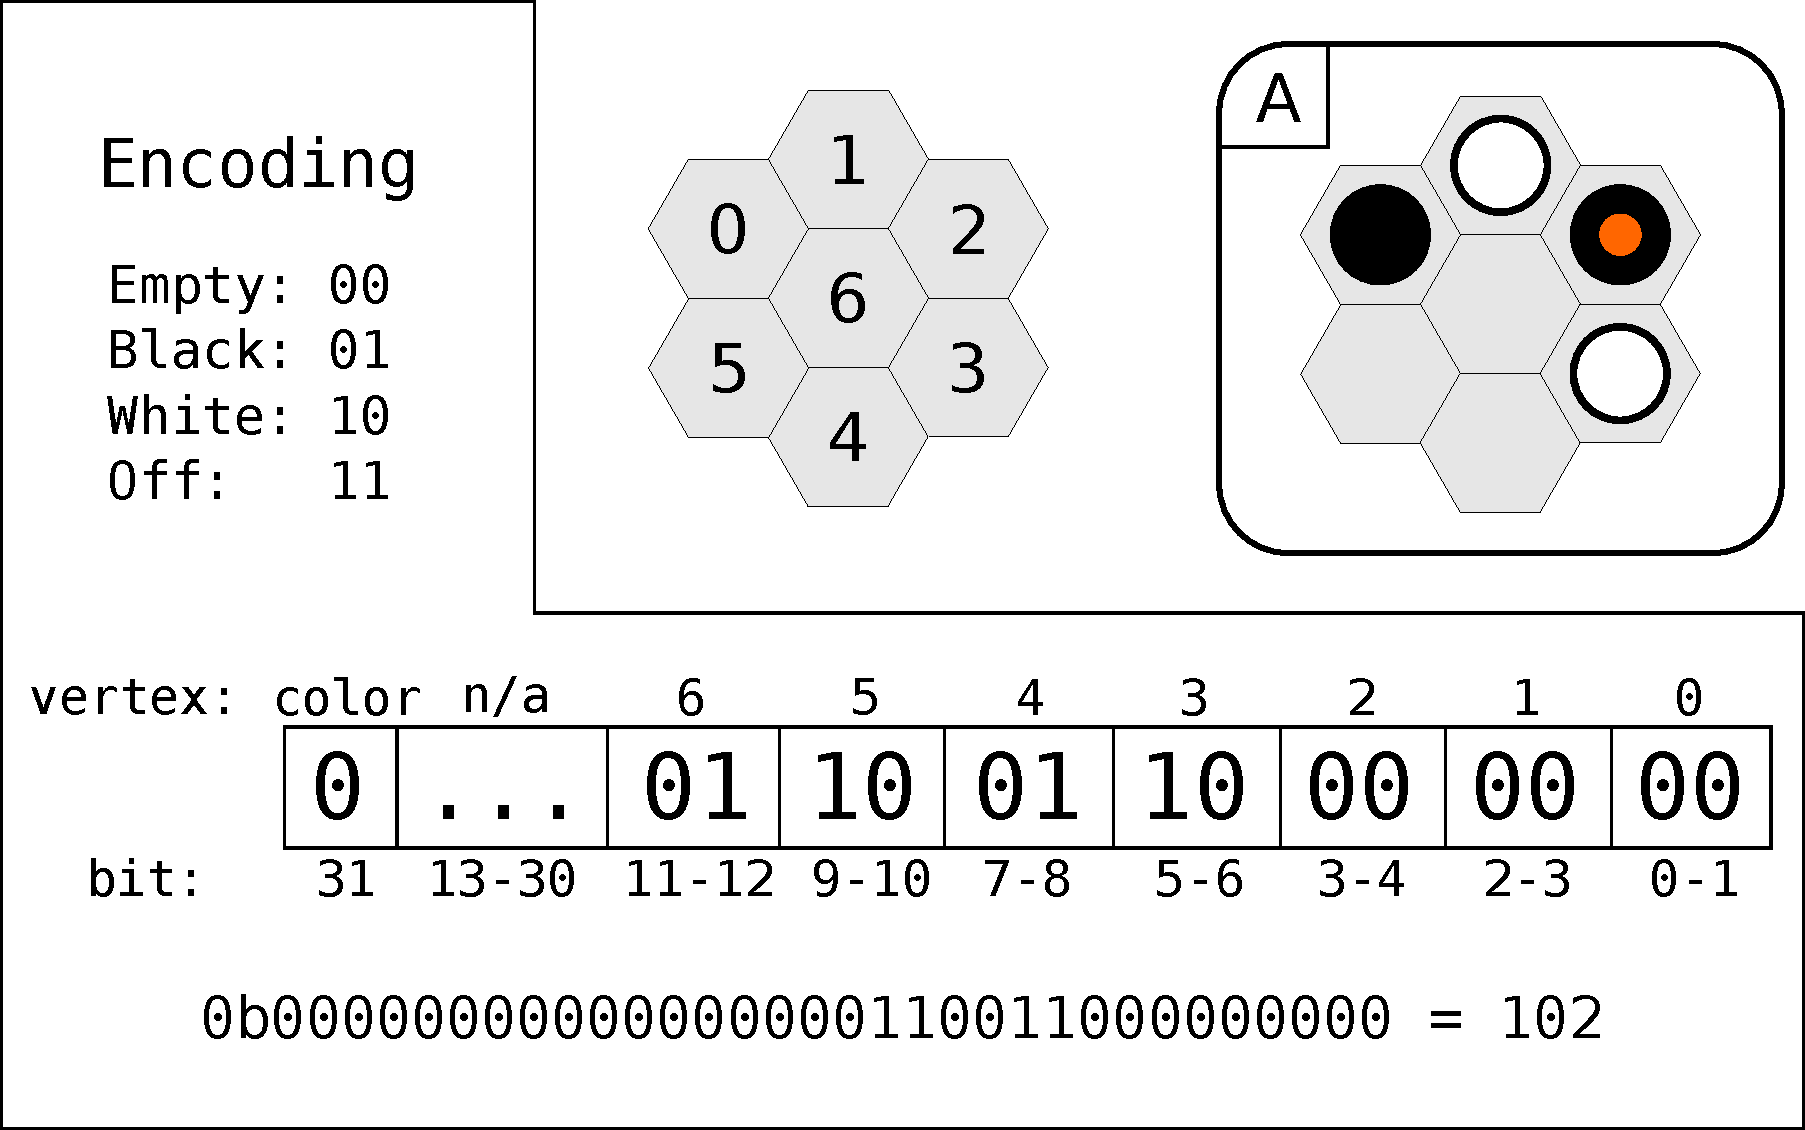
\includegraphics[width=3.25in]{graphics/weight-pattern-map.pdf}
  \label{fig:encoding}
  \end{center}
\end{figure}
\begin{itemize}
	\item Map from 32-bit integer to floating point weight
	\item Evolution (mutation/recombination) operates on individual's map entries
\end{itemize}
\end{frame}

\begin{frame}{Results (Self)}
\begin{figure}
	\begin{center}
		\begin{tabular}{c | c c c}
		& \multispan{3}{\hfil opponent \hfil} \\
		 player & default & uniform & uniform (tenuki) \\
		\hline
		uniform & 70.50\% & & \\
		uniform (tenuki) & 61.00\% & 50.00\% & \\
		learned & 90.00\% & 84.00\% & 86.00\% \\
		\end{tabular}
	\label{fig:results}
	\end{center}
\end{figure}
All-play-all tournament of the 4 Hivemind variants.

Each element is the percent win-rate of the row variant versus the column variant.
\end{frame}

\begin{frame}{Results (Self)}
\centerline{
\begin{tabular}{c | cc cc}
 & \multispan{2}{\hfil default \hfil} & \multispan{2}{\hfil uniform local\hfil} \\
 & 11x11 & 13x13 & 11x11 & 13x13 \\ \hline
 learned win \%	& 92.5 \% & 94 \%  & 88.5\% & 85\% 
 \end{tabular}
}
\end{frame}

\begin{frame}{Results (MoHex 7x7)}
\centerline{
\begin{tabular}{lccc}
& Learned policy & Uniform local & Default policy \\
win \% & 42\% & 26\% & 11.75\%
\end{tabular}
}
\end{frame}

\begin{frame}{Results (MoHex 11x11)}
\centerline{
		\begin{tabular}{c  | c c c}
		Hivemind & Win-rate & Relative CPU \\
		\hline
		Default & 0.5\% & 510\% \\
		Local & 0.0\% & 545\% \\
		Learned & 11\% & 620\% \\
		\end{tabular}
}
\end{frame}

\begin{frame}{Future Work}
\begin{itemize}
	\item Different encodings
	\item General game play
	\item Encode expert knowledge in weights
\end{itemize}
\end{frame}

\end{document}
